\documentclass{beamer}
\newcommand\measurepage{\dimexpr\pagegoal-\pagetotal-\baselineskip\relax}
\title{Team W - Algorithms for Sports Eliminations}
\author{
    Gordon Reid: 1002536R\\
    Ryan Wells: 1002253W\\
    Kris Stewart: 1007175S\\
    David Selkirk: 1003646S\\
    James Gallagher: 0800899G\\
    Dr David Manlove: Project Supervisor
}
\date{March 19, 2013}
\begin{document}
\frame{\titlepage}
\frame{\tableofcontents}
\section{Project outline}
\section{Project results}
\subsection{Algorithm}
\subsection{Parser}
\subsection{Desktop User Interface}
\subsection{Web Application}
\section{Conclusion}
\subsection{Lessons Learnt and Future Work}
\subsection{Project Conclusion}
%"Presentations should describe the aims and objectives of the project, the
%work you have undertaken and the resulting product, the key design and
%management decisions you made, and any lessons learnt. Tell us what you’ve
%done, why it was interesting, what you learnt, what you’d do differently if you
%had to do it again, etc."
\frame{
  \frametitle{Project outline}
  \begin{itemize}
  \item<2-> Aim of the project was to implement an algorithm that
  can mathematically deduce if a team X is eliminated from a Baseball league.
  \item<3-> A team X is only eliminated if there is no mathematically possible
  way for X to finish top of the league.
  \item<4-> Ford-Fulkerson algorithm.
  \item<5-> Builds on na\"{\i}ve calculations made by sports pundits.
  \item<6-> Real world application of Graph Theory.
  \end{itemize}
}
\frame{
  \frametitle{Example}
  \begin{center}
  \begin{figure}
  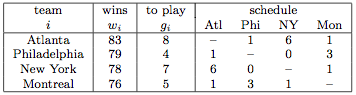
\includegraphics[width=\textwidth]{Example.png}
  \end{figure}
  \tiny{Image courtesy of Kevin D. Wayne, Princeton University}
  \end{center}
}
\frame{
  \frametitle{Algorithm}
  \pause
  \begin{itemize}
  \item<2-> Revolves around creation of directed graphs and flow
    through directed graphs.
  \item<3-> Pushing flow through a specific graph will allow us to
    determine if the given team X is eliminated from a given league.
  \item<4-> A team X can win the league if it is possible for there to
    be a saturating flow. A flow is saturated if the total flow from
    the source equals the total capacity from the source.
  \item<5-> All flow leaving the source has to arrive at the sink.
  \end{itemize}
}
\frame{
  \frametitle{Algorithm - Graph}
  \begin{center}
  \begin{figure}
  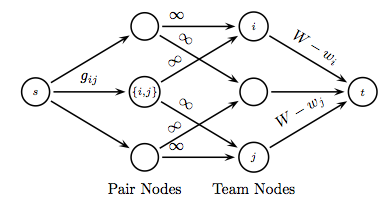
\includegraphics[width=0.4\textwidth]{graph.png}
  \end{figure}
  \tiny{Image courtesy of Kevin D. Wayne, Princeton University}
  \end{center}
}
\frame{
  \frametitle{Algorithm - Extensions}
  \begin{itemize}
    \item<2-> Leauge Elimination by Binary Search Computation
    \item<3-> Certificate of Elimination
    \item<4-> First non-trivially eliminated team
  \end{itemize}
}
\frame{
  \frametitle{Parser}
  \pause
  \begin{center}
  \begin{figure}
  %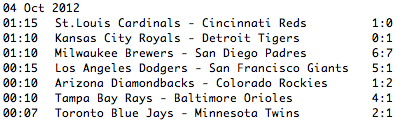
\includegraphics[width=\textwidth]{textfile.png}
  \end{figure}
  \end{center}
  \begin{itemize}
  \item<2-> Uses basic string comparison to put the relevant team in the
  correct League and Division.
  \item<3-> Have considered future plans to parse a web page.
  \item<4-> Our current source is not suitable for real-time updating.
  \item<5-> As a team we are unsure if we would like to implement this feature
  or concentrate our energies on other features for example, making a web-based
  UI.
  \end{itemize}
}
\frame{
  \frametitle{User Interface}
  \begin{itemize}
  \item<2-> User is likely an advanced follower of the sport looking for
  very specific information.
  \item<2-> Simple design based on presenting this key information immediately.
  \item<3-> More detailed information available on user request.
  \item<4-> Challenge is to integrate the two tasks such that the UI is
  both functionally and aesthetically pleasing.
  \end{itemize}
}
\frame{
  \frametitle{User Interface - Key Tasks}
  \begin{itemize}
  \item<1-> Display all teams by division and league, showing elimination status.
  \item<2-> Update the elimination status on start-up.
  \item<3-> Display certification of elimination for teams eliminated.
  \end{itemize}
}
\frame{
  \frametitle{User Interface - Prototype}
  \begin{figure}
  %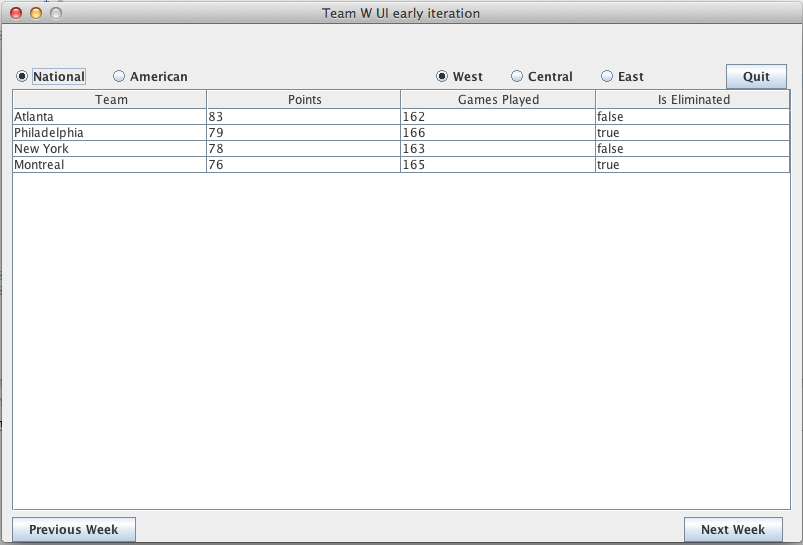
\includegraphics[width=\textwidth]{InitialUI.png}
  \end{figure}
}
\frame{
  \frametitle{User Interface - Additional Tasks}
  \begin{itemize}
  \item<1-> Allow date navigation, displaying correct results for each the date.
  \item<2-> Display print functionality.
  \item<3-> Display league generation functionality.
  \end{itemize}
}
\frame{
  \frametitle{User Interface - Final}
  \begin{figure}
  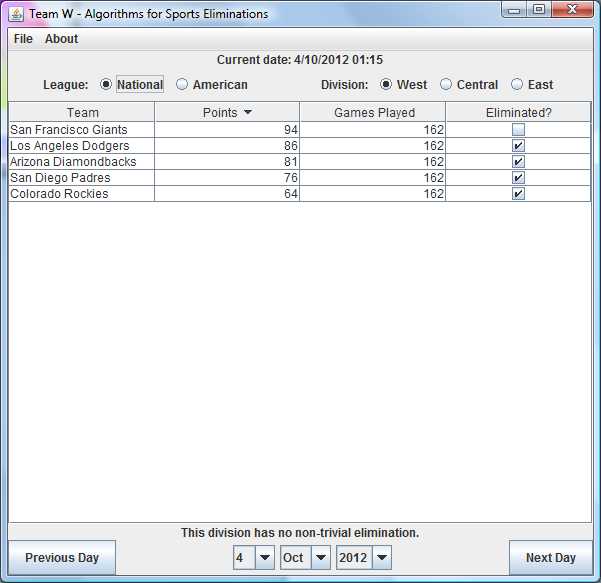
\includegraphics[scale=0.4,keepaspectratio]
  {finalDesktopUI.png}
  \end{figure}
}
\frame {
  \frametitle{Web Application}
  \begin{itemize}
  \item<2-> An extension of the project.
  \item<2-> Contains a subset of most important functionality of
  desktop application.
  \item<2-> Numerous extensions of web application part of future work.
  \end{itemize}
}
\frame {
  \frametitle{Web Application Screenshot}
  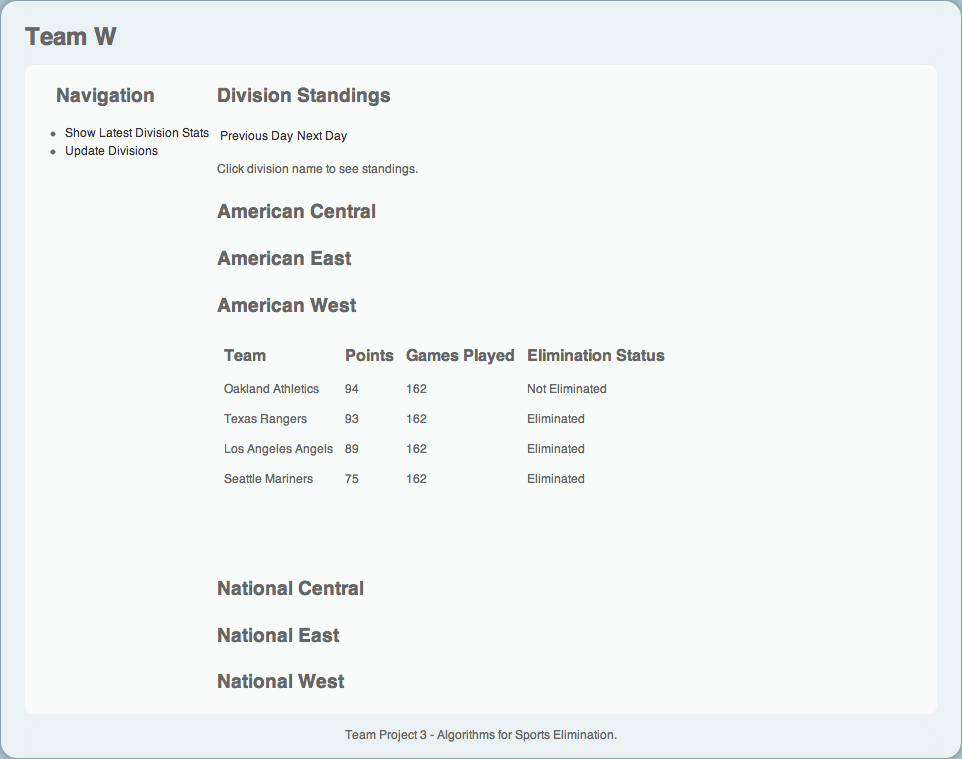
\includegraphics[width=\textwidth,height=\measurepage,keepaspectratio]
  {webAppScreenshot.png}
}
\frame {
  \frametitle{Lessons Learnt and Future Work}
  \begin{itemize}
  \item
  \end{itemize}
}
\frame {
  \frametitle{Project Conclusion}
  \begin{itemize}
  \item Successfully implemented all must have functionality.
  \item Fun and interesting to take theory and implement real-world application.
  \item Informative user evaluation.
  \item Plenty of scope for future work.
  \end{itemize}
}
\frame {
  We would now like to invite questions from the panel.

  Thank you for listening.
}
\end{document}
